%% discuss techniques and refer to previous examples (message: it depends when what is feasible)
%\subsection{S1: Exclude Feature Combinations}
%% example: leonovo option compatibility matrix (even if not strictly enforced)
%% example: web configurators (Thinkpad)
%\subsection{S2: Orthogonal Implementation}
%\subsection{S3: Duplicate Implementations}
%\subsection{S4: Move Source Code}
%\subsection{S5: Preprocessors}
%\subsection{S6: Derivative Modules}
%\subsection{Overview on all Strategies}
%\subsection{When to Handle?}
%% spreadshirt example: fixing foreground+background colors for every order


\subsection{Motivation}

\begin{frame}{Handling/Implementing Feature Interactions}
	\begin{mycolumns}[widths={50,50},animation=none]
		\mynote{Assumptions}{
			\begin{itemize}
				\item Interacting features have been already identified
				\item Interaction is a pairwise interaction (i.e., two features)
			\end{itemize}
		}
	\mynextcolumn
		\mydefinition{Problem Description}{
			\begin{itemize}
				\item Find a strategy to handle the interaction 
				\item Strategy does not introduce the optional-feature problem
			\end{itemize}
		}
	\end{mycolumns}
\end{frame}

\begin{frame}[fragile]{Example: A Feature Interaction in our Graph Library}
	\begin{mycolumns}[widths={50,50},animation=none]
		\myexampletight{}{
			\centering
			\featureDiagram{
				Graph,concrete
				[Nodes,mandatory,abstract
					[Colored,optional,concrete]]
				[Edges,mandatory,abstract
					[Directed,optional,concrete]
					[Weighted,optional,concrete]]
				[Algorithms,mandatory,abstract,
					[ShortestPath,optional,concrete]]
			}
		}
		\vspace{3mm}
		\mynote{}{
			\begin{itemize}
				\item Domain view: $Weighted$ and $ShortestPath$ can be deliberately selected independent of each other.
				\item Implementation view: $ShortestPath$ requires $Weighted$ due to an implementation dependency (optional-feature problem!).
			\end{itemize}
		}
	\mynextcolumn
{\small
\begin{codetight}{layer: BasicGraph}
class Edge {
	private Node a, b;
	...
}
\end{codetight}	
\begin{codetight}{layer: Weighted}
refines class Edge {
	double weight;
	void setWeight(double w){ ... }
}
\end{codetight}	
\begin{codetight}{layer: ShortestPath}
refines class Graph {
	List shortestPath(Node a, Node b){
		Edge e1, e2;
		...
		if(e1.weight > e2.weight) 
		... 
	}
}
\end{codetight}	
}
	\end{mycolumns}
\end{frame}

\begin{frame}{Handling/Implementing Feature Interactions: General Goals}
	\mynote{Question}{
		What makes a good strategy to implement coordination code for feature interactions (while solving/avoiding the optional-feature problem)?
	}
	\pause
	\begin{mycolumns}[widths={50,50},animation=none]
		\mydefinition{1. Variability}{
			For every valid configuration (according to feature model), we can generate a product that implements this configuration.
		}
		\pause
		\mydefinition{2. Implementation effort}{
			Should not require overwhelming implementation effort (would not be attractive in practice).
		}
		\pause
	\mynextcolumn
		\mydefinition{3. Binary size and performance}{
			Should not increase binary size or decrease performance of products compared to an individual implementation of each product.
		}
		\pause
		\mydefinition{4. Code quality}{
			Should not reduce code quality, which would make the product line harder to maintain. 
		}
		\pause
	\end{mycolumns}
\end{frame}

\subsection{S1: Adapt Feature Model}

\begin{frame}{S1 (a): Adapt Feature Model - Add Domain Dependency}
	\mydefinition{Strategy}{
		Declare implementation dependency as domain dependency in the feature model.
	}
	\mynotetight{}{
		\centering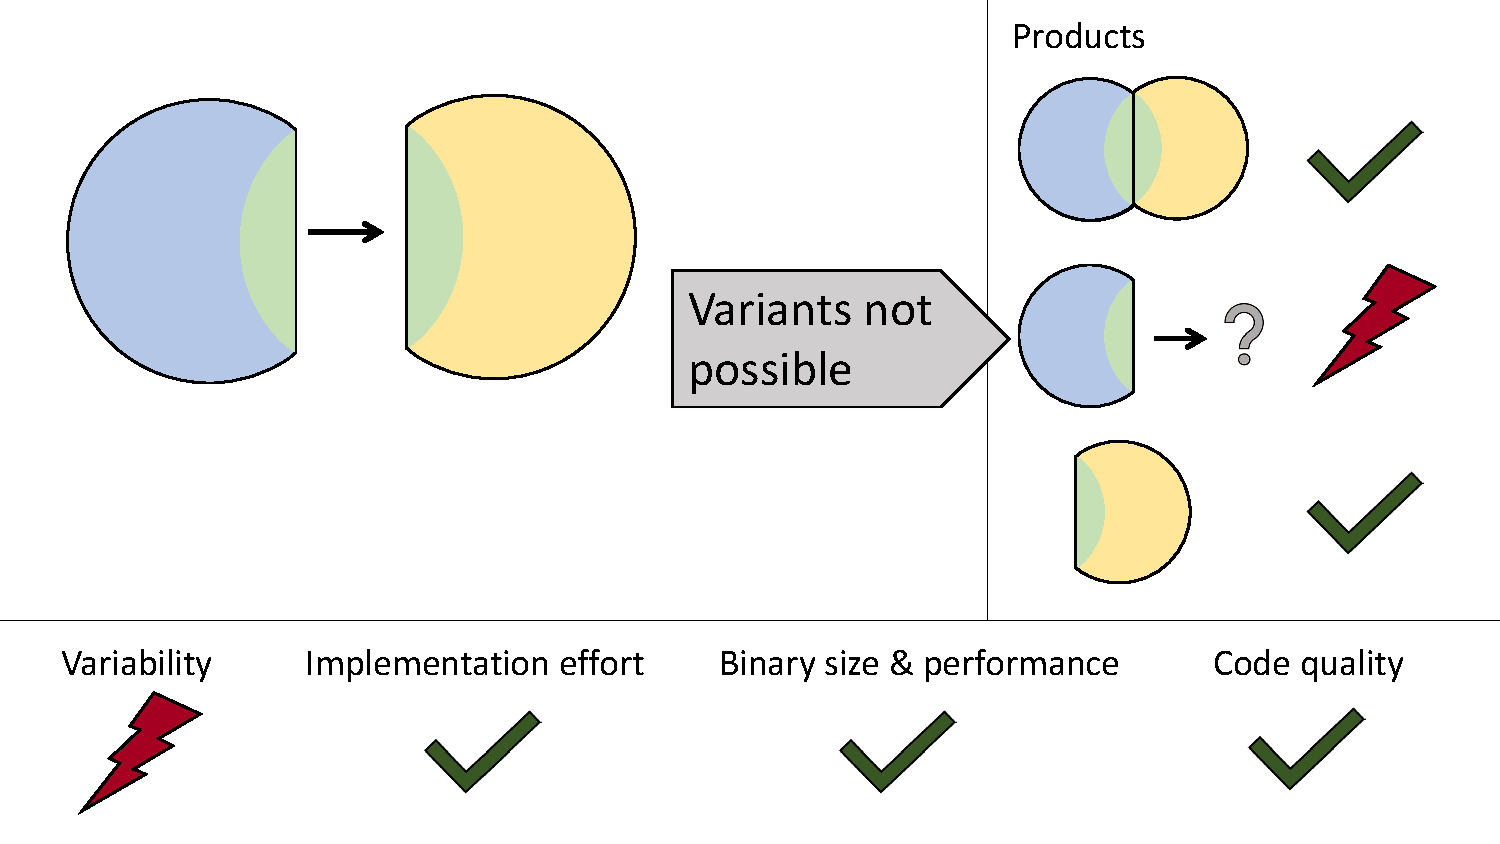
\includegraphics[width=0.7\linewidth,page=1]{interaction-handling}
	}
\end{frame}

\begin{frame}[fragile]{Example}
	\begin{mycolumns}[widths={50,50},animation=none]
		\myexampletight{}{
			\centering
			\featureDiagram{
				Graph,concrete
				[Nodes,mandatory,abstract
					[Colored,optional,concrete]]
				[Edges,mandatory,abstract
					[Directed,optional,concrete]
					[Weighted,optional,concrete]]
				[Algorithms,mandatory,abstract,
					[ShortestPath,optional,concrete]]
			}

			$ShortestPath \pimplies Weighted$  
		}
		\vspace{3mm}
		\mynote{}{
			Same implementation as before, but we make implementation dependency explicit: $ShortestPath$ requires $Weighted$.
		}
	\mynextcolumn
{\small
\begin{codetight}{layer: BasicGraph}
class Edge {
	private Node a, b;
	...
}
\end{codetight}	
\begin{codetight}{layer: Weighted}
refines class Edge {
	double weight;
	void setWeight(double w){ ... }
}
\end{codetight}	
\begin{codetight}{layer: ShortestPath}
refines class Graph {
	List shortestPath(Node a, Node b){
		Edge e1, e2;
		...
		if(e1.weight > e2.weight) 
		... 
	}
}
\end{codetight}	
}
	\end{mycolumns}
\end{frame}

\begin{frame}{S1 (b): Adapt Feature Model - Exclude Feature Combinations}
	\mydefinition{Strategy}{
		Declare problematic feature combinations as mutually exclusive in the feature model.
	}
	\mynotetight{}{
		\centering\includegraphics[width=0.7\linewidth,page=2]{interaction-handling}
	}
\end{frame}

\begin{frame}[fragile]{Example}
	\begin{mycolumns}[widths={50,50},animation=none]
		\myexampletight{}{
			\centering
			\featureDiagram{
				Graph,concrete
				[Nodes,mandatory,abstract
					[Colored,optional,concrete]]
				[Edges,mandatory,abstract
					[Directed,optional,concrete]
					[Weighted,optional,concrete]]
				[Algorithms,mandatory,abstract,
					[ShortestPath,optional,concrete]]
			}

			$\pnot (ShortestPath \pand Weighted)$  
		}
		\vspace{3mm}
		\mynote{}{
			We may safely assume any uniform weight because $ShortestPath$ and $Weighted$ are mutually exclusive.
		}
	\mynextcolumn
\vspace{-3mm}
{\small
\begin{codetight}{layer: BasicGraph}
class Edge {
	private Node a, b;
	...
}
\end{codetight}	
\begin{codetight}{layer: Weighted}
refines class Edge {
	double weight;
	void setWeight(double w){ ... }
}
\end{codetight}	
\begin{codetight}{layer: ShortestPath}
refines class Graph {
	List shortestPath(Node a, Node b){
		@float w1 = 1.0;@
		@float w2 = 1.0;@
		...
		@if(w1 > w2)@
		... 
	}
}
\end{codetight}	
}
	\end{mycolumns}
\end{frame}

\subsection{S2: Orthogonal Implementation}

\begin{frame}{\myframetitle}
	\mydefinition{Strategy}{
		Orthogonal implementation with no dedicated coordination of interaction.
	}
	\mynotetight{}{
		\centering\includegraphics[width=0.7\linewidth,page=3]{interaction-handling}
	}
\end{frame}

\begin{frame}[fragile]{Example}
	\begin{mycolumns}[widths={50,50},animation=none]
		\myexampletight{}{
			\centering
			\featureDiagram{
				Graph,concrete
				[Nodes,mandatory,abstract
					[Colored,optional,concrete]]
				[Edges,mandatory,abstract
					[Directed,optional,concrete]
					[Weighted,optional,concrete]]
				[Algorithms,mandatory,abstract,
					[ShortestPath,optional,concrete]]
			}

			$\pnot (ShortestPath \pand Weighted)$  
		}
		\vspace{3mm}
		\mynote{}{
			Calculation of shortest path ignores weights but merely counts the number of edges on a path.
		}
	\mynextcolumn
{\small
\begin{codetight}{layer: BasicGraph}
class Edge {
	private Node a, b;
	...
}
\end{codetight}	
\begin{codetight}{layer: Weighted}
refines class Edge {
	double weight;
	void setWeight(double w){ ... }
}
\end{codetight}	
\begin{codetight}{layer: ShortestPath}
refines class Graph {
	List shortestPath(Node a, Node b){
		@// ignore weights@
		... 
	}
}
\end{codetight}	
}
	\end{mycolumns}
\end{frame}

\subsection{S3: Duplicate Implementations}

\begin{frame}{\myframetitle}
	\mydefinition{Strategy}{
		Multiple implementations of a feature, with and without coordination code.
	}
	\mynotetight{}{
		\centering\includegraphics[width=0.7\linewidth,page=4]{interaction-handling}
	}
\end{frame}

\begin{frame}[fragile]{Example}
	\begin{mycolumns}[widths={50,50},animation=none]
\begin{codetight}{layer: ShortestPath\_Unweighted}
refines class Graph {
	List shortestPath(Node a, Node b){
		...
		...
		// ignore weights
		... 
	}
}
\end{codetight}
		\mynote{}{			
			Selected iff $ShortestPath \pand \pnot Weighted$. 
		}
	\mynextcolumn
\begin{codetight}{layer: ShortestPath\_Weighted}
refines class Graph {
	List shortestPath(Node a, Node b){
		Edge e1, e2;
		...
		if(e1.weight > e2.weight) 
		... 
	}
}
\end{codetight}	
		\mynote{}{
			Selected iff $ShortestPath \pand Weighted$.
		}
	\end{mycolumns}
\end{frame}

\subsection{S4: Move Source Code}

\begin{frame}{\myframetitle}
	\mydefinition{Strategy}{
		Move all the coordination code to one of the features (or to a third one all interacting features depend on).
	}
	\mynotetight{}{
		\centering\includegraphics[width=0.7\linewidth,page=5]{interaction-handling}
	}
\end{frame}

\begin{frame}[fragile]{Example}
	\begin{mycolumns}[widths={50,50},animation=none]
\begin{codetight}{layer: BasicGraph}
class Edge {
	private Node a, b;
	@double weight = 1.0;@
	...
}
\end{codetight}	
\begin{codetight}{layer: Weighted}
refines class Edge {
	void setWeight(double w){ ... }
}
\end{codetight}	
	\mynextcolumn
\begin{codetight}{layer: ShortestPath}
refines class Graph {
	List shortestPath(Node a, Node b){
		Edge e1, e2;
		...
		if(e1.weight > e2.weight) 
		... 
	}
}
\end{codetight}	
	\end{mycolumns}
\end{frame}

\subsection{S5: Conditional Compilation}

\begin{frame}{\myframetitle}
	\mydefinition{Strategy}{
		Coordination code is only executed if both features are selected.
	}
	\mynotetight{}{
		\centering\includegraphics[width=0.7\linewidth,page=6]{interaction-handling}
	}
\end{frame}

\begin{frame}[fragile]{Example: A Feature Interaction in our Graph Library}
	\begin{mycolumns}[widths={50,50},animation=none]
\begin{codetight}{layer: BasicGraph}
class Edge {
	private Node a, b;
	...
}
\end{codetight}	
\begin{codetight}{layer: Weighted}
refines class Edge {
	double weight;
	void setWeight(double w){ ... }
}
\end{codetight}	
	\mynextcolumn
\begin{codetight}{layer: ShortestPath}
refines class Graph {
	List shortestPath(Node a, Node b){
		Edge e1, e2;
		...
@#ifdef WEIGHTED@		
		if(e1.weight > e2.weight) ...
@#endif@
		... 
	}
}
\end{codetight}	
	\end{mycolumns}
\end{frame}

\subsection{S6: Derivative Modules}

\begin{frame}{\myframetitle}
	\mydefinition{Strategy}{
		Create a dedicated module for code that coordinates features.
	}
	\mynotetight{}{
		\centering\includegraphics[width=0.7\linewidth,page=7]{interaction-handling}
	}
\end{frame}

\begin{frame}[fragile]{Example: A Feature Interaction in our Graph Library}
	\begin{mycolumns}[widths={50,50},animation=none]
\begin{codetight}{layer: ShortestPath}
refines class Graph {
	List shortestPath(Node a, Node b){
		Edge e1, e2;
		...
		if(isLonger(e1,e2)) 
		... 
	}
	boolean isLonger(Edge e1, Edge e2){
		return false;
	}
}
\end{codetight}	
	\mynextcolumn
\begin{codetight}{layer: ShortestPath\_Weighted}
refines class Graph {
	boolean isLonger(Edge e1, Edge e2){
		return e1.weight > e2.weight;
	}
}
\end{codetight}	
		\mynote{}{			
			Selected iff $ShortestPath \pand Weighted$. 
		}	
	\end{mycolumns}
\end{frame}

\subsection{Overview and Discussion}

\begin{frame}{Overview and Discussion}
	\centering\includegraphics[width=0.9\linewidth,page=8,trim=40 25 40 25,clip]{interaction-handling}
\end{frame}


